\RequirePackage{fix-cm}

%
%\documentclass{svjour3}                     % onecolumn (standard format)
%\documentclass[smallcondensed]{svjour3}     % onecolumn (ditto)
%\documentclass[smallextended]{svjour3}       % onecolumn (second format)
\documentclass[twocolumn]{cgi2015_latex/svjour3}          % twocolumn
\smartqed  % flush right qed marks, e.g. at end of proof
\usepackage{graphicx}
\usepackage{amsmath, amssymb}
\journalname{CGI2015} % The correct name will be entered by the editor

\graphicspath{{figures/}}

\begin{document}

\title{Real-time visualisation of volumetric data on the GPU}
\subtitle{}
\author{H. Perrier \and J. Dupuy \and J.-C. Iehl \and J.-P. Farrugia}
\institute{H. Perrier \at helene.perrier@liris.cnrs.fr \and J. Dupuy \at jonathan.dupuy@liris.cnrs.fr \and J.-C. Iehl \at jean-claude.iehl@liris.cnrs.fr \and J.-P. Farrugia \at jean-philippe.farrugia@liris.cnrs.fr}
\date{ }% The correct dates will be entered by the editor

\maketitle

\begin{figure}
\centering
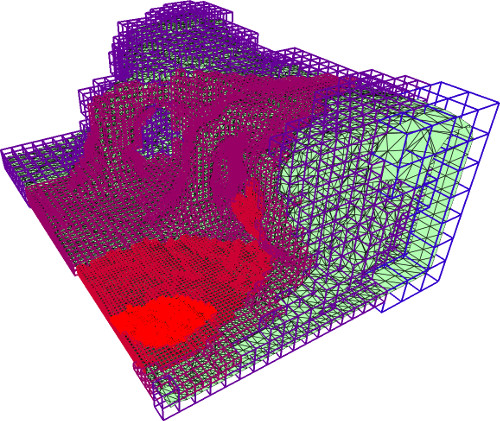
\includegraphics[width=0.7\linewidth]{octree}
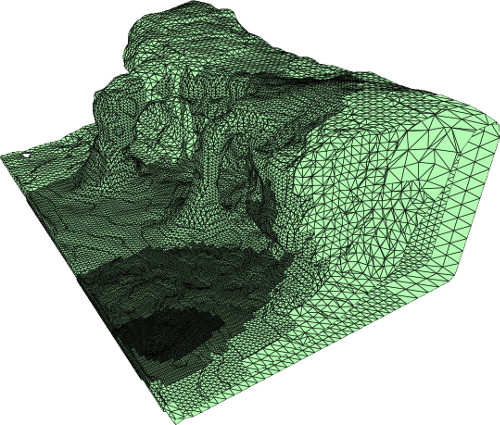
\includegraphics[width=0.7\linewidth]{mesh_muti_res}
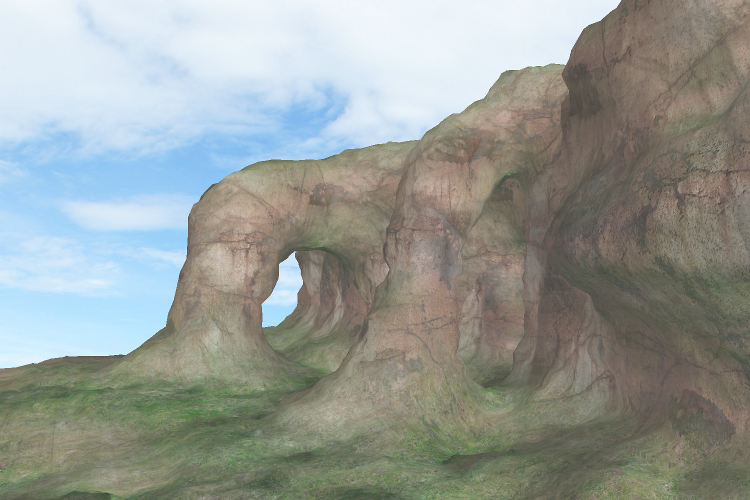
\includegraphics[width=0.7\linewidth]{terrain_potential}
\caption{Our method is based on Lengyel's algorithm \cite{lengyel2010voxel} combined with a linear restricted octree (top) which allows us to create adaptive meshes (middle) from volumetric data in real-time (bottom).}
\end{figure}

\begin{abstract}
We present a tool to visualise volumetric data in real-time by extracting an adaptive triangulated surface from the object.
We extend an existing adaptive marching cubes solution and increase its execution speed by developing a pipeline that is fully data parallel and implemented on the GPU.
This lets us visualise in real-time static scenes as well as fully dynamic data.
Furthermore, we propose a criterion to control the adaptivity of the triangulation that adds control over the projected size of triangles.
This allow us to remove geometric aliasing in the resulting rendering.
\keywords{GPU, Real-time, Level of Details, Volumetric Datasets}
\end{abstract}

\section{Introduction} 

\paragraph{} %Intro générale
Volumetric objects are being more and more used in computer graphics.
They represent a volume by a function that associate a density to each point in world space.
This function can be defined analytically or with a dataset.
Since this representation does not contain topological information, volumetric objects are easy to manipulate.
They are hence a good candidate for procedural generation \cite{peytavie2009arches}.
They can be also be found in medical applications, considering they are the output of acquisition scanners.
Finally, this representation is widely used in gas and fluids simulation \cite{bridson2007fluid}.


\paragraph{} %Nos conditions pour assurer cette visualisation correcte
Visualising such objects is a crucial issue.
However, it imposes several constraints.
For interactive applications, it must be done in real-time.
We must also be able to render dynamic datasets such as fluids, as well as changing on the fly the data parameters.
Furthermore, visualising the results should be done as fast as possible to leave computational time for simulation purposes.
A solution would be to have a full GPU implementation that runs asynchronously from the CPU.
To sum up, an ideal method would fulfill those conditions:
\begin{itemize}
	\item Able to visualise volumetric objects in real-time.
	\item Able to handle dynamic datasets.
	\item Implemented entirely on the GPU.
\end{itemize}

\paragraph{}
There are two families of solutions to visualise volumetric data in real-time : ray casting and rasterization.
Ray casting  \cite{hadwiger2005real} accounts easily for lighting effects.
It also renders easily transparent surfaces, which can be useful when visualising medical datasets.
However, it does not fit the GPU pipeline and is thus slower than rasterization based solutions.

\paragraph{}
Our goal is to implement a solution that runs as fast as possible by taking full advantage of the GPU hardware. 
We thus choose to use rasterization.
This implies that a triangulated surface needs to be extracted from the data.
A very popular algorithm to do this triangulation is Marching Cubes (MC) \cite{lorensen1987marching}. 
It is data parallel so a GPU implementation of this method is very efficient \cite{tatarchuk2007real}.
During the rasterization process, each pixel of the framebuffer samples a unique triangle.
As a result, when several triangles project onto the same pixel, aliasing artefacts appear due to under-sampling (Figure \ref{lod}). 
To avoid such artefacts, the surface extraction must be adaptive to maintain a good sampling rate.

%\begin{figure}
%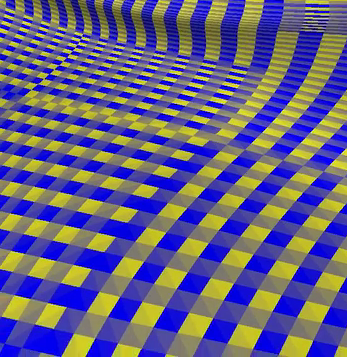
\includegraphics[height=0.125\textheight]{alias_close}
%\hfill
%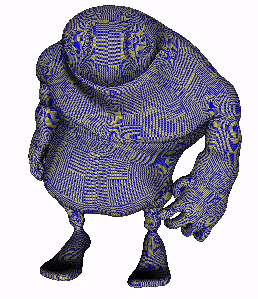
\includegraphics[height=0.125\textheight]{alias_far}
%\hfill
%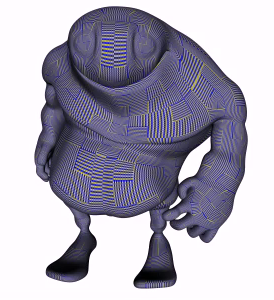
\includegraphics[height=0.125\textheight]{groundtruth}
%\caption{This model has a different color for each of its triangles. When close (Left), every triangle projects onto more than a pixel so the visualisation is fine. When viewed from distance (Middle), several triangles projects onto a single pixel and aliasing artefacts occur. (Right) is the same object visualised with 1024 samples per pixel.}
%\label{aliasing}
%\end{figure}

\paragraph{} %Situation par rapport au STAR
We are thus facing a problem of adaptive surface extraction, which is an extensively studied topic.
Many solutions have been developed in computational geometry \cite{shu1995adaptive,schaefer2004dual}.
However, they focus on the topology of the resulting mesh, whereas we focus on correct visualisation.
Real-time solutions have been developed using Level of Details (LoD). 
These methods dynamically refine the extracted triangulation using both the curvature of the object and its distance to the camera.
But since they rely on a preprocessing phase, they do not support visualising fully dynamic data in real-time.

\paragraph{}
Most of those LoD solutions were developed for heightfields visualisation \cite{duchaineau1997roaming}.
Yet, there are solutions that triangulate true volumetric data by applying MC on a hierarchical partition of space.
Since MC is not adaptive, the resulting hierarchical triangulation may carry cracks at resolution changes.
To avoid this, complex structures \cite{scholz2014real,schaefer2004dual} may be used or more triangles may be generated to stitch the holes \cite{lengyel2010voxel}.
Such adaptive methods run in real-time but they require both CPU and GPU time.
Furthermore, for performance purposes, some of them cache parts of the triangulation, which prevents the use of fully dynamic data.
Finally, none of the aforementioned solutions ensure a minimal triangle size, and are thus subject to aliasing issues.

\paragraph{} %What we do
The method developed by Lengyel \textit{et al.} \cite{lengyel2010voxel} is the best suited to our needs.
However, it was preferably developed to visualise in real-time static or near static data and present a complex CPU implementation.
In this paper we propose a GPU pipeline inspired from this method.
It leaves the CPU free for other tasks and avoids synchronisation with the GPU.
Our high framerate also allows this method to run in real-time on fully dynamic data. 
The triangulation is controlled by a GPU LoD criterion that ensures that triangles project onto more than one pixel, thus removing geometrical aliasing.

\paragraph{}
In the next section, we present the main algorithms on which our work is based \cite{lengyel2010voxel,dupuy2014quadtrees}. 
Then, we present our GPU implementation, followed by our results and performances.
Finally, we end up by concluding on the limitations and perspectives of our approach.

%p1 : pourquoi volumes cools et important de les visu
%p2 : nos contraintes et pk celles là
%p3 : les methodes actuelles ac leurs objectifs !=
%p4 : ce qu'on fait
%p5 : plan

\section{Background}

The solution of Lengyel \textit{et al.} \cite{lengyel2010voxel} is
based on extracting an adaptive triangulated surface by applying MC on
an octree.  However, due to its recursive nature, the octree is not
suited for the GPU pipeline.  Hence, to take full advantage ofthe GPU,
we must convert this tree to a non recursive structure.  Such
representations were first introduced by Gargantini
\cite{gargantini1982effective} and are known as linear quadtrees.
They have been implemented on the GPU by Dupuy \textit{et al.}
\cite{dupuy2014quadtrees}.  Along with this implementation, they
presented a LoD criterion that bounds the projected size of the tree
cells.

\subsection{Adaptive surface extraction}

\begin{figure}
\centering
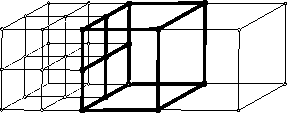
\includegraphics[width=0.8\linewidth]{transition_cell}
\caption{ Triangulating a hierarchical grid with MC creates cracks at level changes.
To fix those, Lengyel \textit{et al}. inserts transition cells (bold).
Those cells are more subdivided on one side to patch the change of resolution.}
\label{transition_cell}
\end{figure}


\paragraph{}
Lengyel \textit{et al}. \cite{lengyel2010voxel} developed a solution to visualise volumetric data in real-time.
They start by subdividing the space with an octree.
At each frame, they select a set of cells within this tree, called the active front, that partitions the space.
The resolution of the partition varies along the space, depending on the chosen cells.
This idea is illustrated for quadtrees in the Figure \ref{fig_quadtree_partitionning}.
Whether a cell is part of this active front is determined by evaluating a LoD criterion.
The selected cells can finally be triangulated using a method similar to MC.

\paragraph{}
When two cells of different resolution meet, T-Junctions appear.
They are due to some vertices in the high resolution cells that have no match in the low resolution cell.
The problem is that when using a MC algorithm, those inconsistencies create cracks in the final triangulation.
To fix this, Lengyel \textit{et al.} inserts transition cells (Figure \ref{transition_cell}) where two cells of different level meet.
Those cells are more subdivided one on side than on the other to patch the difference of resolution.
They are then triangulated with a modified MC, producing a crack-free surface for visualisation.
However, it requires having triangulation tables adapted to the unusual structure of the transitions.
It also demands the use of a restricted octree, since the transitions only allow a single level of difference between neighbouring cells.
As the triangulation is based on modified MC, it is data parallel.

\paragraph{}
The adaptivity of the final triangulation is controlled by a LoD criterion.
Lengyel \textit{et al}. use a measure based on the distance between the cell and the camera, which must therefore be re-evaluated every time the camera moves.

\paragraph{}
On the GPU, recomputing the whole active front from the root node would be too expensive.
Instead, we update the tree by merging or splitting the cells.
If this operation could be done on the GPU, it would be possible to extract the adaptive triangulation entirely on the GPU.
This requires a non recursive representation for the tree, as well as data parallel update operations.
The LoD must also be evaluable during a data parallel process as it controls the partition.
Those properties can be found using linear trees \cite{dupuy2014quadtrees}.


\subsection{Linear Quadtrees}

\begin{figure}
\centering
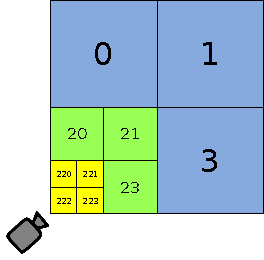
\includegraphics[height=0.17\textheight]{partitioning.pdf}
\hfill
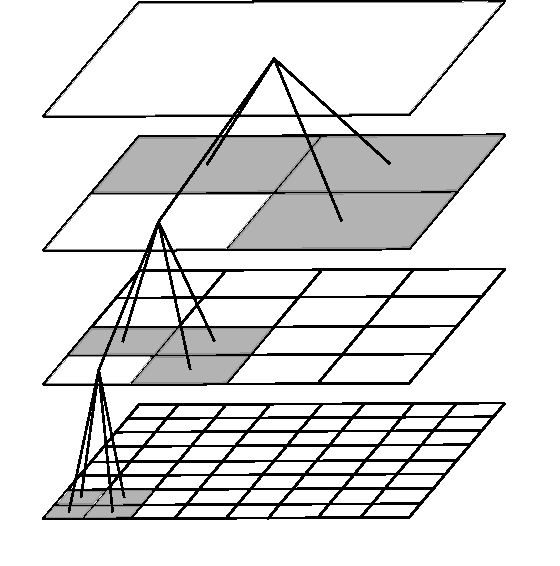
\includegraphics[height=0.17\textheight]{quadtree_activefront}
\caption{In \cite{dupuy2014quadtrees}, a linear quadtree is used to maintain a 2D hierarchical partitioning of space.
(Left) presents such a partitioning.
A cell is more or less subdivided depending on its distance to the camera.
They are also encoded with morton code, that identifies each cell with its position relatively to its parent.
(Right) shows the corresponding active front in the full tree.
This partition is entirely represented by storing the list of codes of the gray cells. }
\label{fig_quadtree_partitionning}
\end{figure}


\paragraph{}
Linear quadtrees were presented by Gargantini \cite{gargantini1982effective} as a non recursive representation for quadtrees.
Such structures were reused by Dupuy \textit{et al.} \cite{dupuy2014quadtrees} who presented a solution to handle them efficiently on the GPU.

\paragraph{}
Linear quadtrees associate a code to each cell, identifying it by its path to the root node.
The full tree is thus entirely represented by the list of its leaves' codes, which removes the recursivity.
In their implementation, Dupuy \textit{et al.} used Morton codes (Figure \ref{fig_quadtree_partitionning}).
Those codes store a spatial position, encoding the location of the cell relatively to its parent.
The final code of a cell is thus the succession of locations between the cell and the root node.
Therefore, the maximal depth of the tree depends on the number of quadrants that can be encoded.
In a quadtree, a cell is divided into $2^2$ quadrants, so encoding one subdivision requires two bits.
Dupuy \textit{et al.} store for each cell its Morton code and its depth within the tree.
Therefore, with a code stored on 32 bits, using 28 bits for the locations and 4 bits for the depth, the tree is limited to 14 levels.

\paragraph{}
Dupuy \textit{et al}. used those quadtrees to maintain a 2D hierarchical space partition.
They thus encode a front of cells within this tree (Figure \ref{fig_quadtree_partitionning}).
To determine if a cell is part of the front, they evaluate on each of them a LoD criterion.
The criterion they chose is view dependent and thus must be evaluated quickly on the GPU.

\paragraph{}
During an update, there a three possible operations on a cell: it can be kept, merged or split.
A merge operation removes the codes of the children's cells from the list and replaces them with the code of the parent cell.
A split operation removes the code of a cell replacing it by the codes of its children.
Therefore, an efficient GPU implementation relies on the fact that those operations can be done independently on each cell.
This is true as long as the LoD criterion is also evaluable independently on each cell.

\paragraph{}
With this implementation of linear tree, it is possible to maintain a quadtree on the GPU.
By generalizing this to the octree, it could be used with the triangulation presented by Lengyel \textit{et al.} to develop a fully data parallel pipeline.
There is however three conditions on the LoD criterion.
It must ensure that the extracted triangles will project onto more than one pixel, to ensure a good rasterization sampling.
The tree must also stay restricted at all times as the transition cells of Lengyel \textit{et al.} only patch cells with a single change in resolution.
Finally, this criterion must allow to detect if the neighbour of a cell is more subdivided than the cell itself in a data parallel manner.
This is mandatory to determine where the transition cells should be inserted.


\subsection{LoD on projected size}

\paragraph{}
When rasterizing a triangulated surface, to ensure a good sampling, all triangles must project onto more than one pixel.
When using a MC algorithm, the size of the generated triangles is bounded by the size of the cell.
Therefore, the cells must all project onto more than one pixel.

\paragraph{}
Dupuy \textit{et al.} \cite{dupuy2014quadtrees} addressed this issue.
They use linear quadtrees to achieve adaptive tessellation.
The subdivision of their quadtree's cells is controlled by a LoD criterion that is evaluable on the GPU and that is based on the cells projected size.
This ensures that all cells project onto more than a pixel.
This criterion is given in equation (\ref{lod_criterion}).
\\
\begin{equation}
s(z) = z \cdot \tan(\alpha)
\label{lod_criterion}
\end{equation}

\paragraph{}
Here, $2 \cdot s(z)$ is the projected screen size at a distance $z$ from the camera, and $2\cdot\alpha$ is the horizontal viewing angle (the fovy). 
To determine if a cell should be merged/split, the ratio $$\frac{\mathrm{cell\_size}}{2 \cdot s(z)}$$ is evaluated.
This ratio is compared to a factor $k$ that controls the density of the triangulation.\\
\begin{equation}
\mathrm{If} \hspace{15pt} \frac{\mathrm{cell\_size}}{2 \cdot s(z)} \geq k \hspace{15pt} \mathrm{then} \hspace{3pt} \mathrm{split}
\label{split_test}
\end{equation}
\begin{equation}
\mathrm{Else} \hspace{3pt} \mathrm{if} \hspace{15pt} \frac{\mathrm{parent\_cell\_size}}{2 \cdot s(z_{\mathrm{parent}})} \leq k \hspace{15pt} \mathrm{then} \hspace{3pt} \mathrm{merge}
\label{merge_test}
\end{equation}
\begin{equation*}
\mathrm{Else} \hspace{3pt} \mathrm{keep}
\end{equation*}
\paragraph{}
Evaluating (\ref{split_test}) splits a cell if its project size exceeds a certain amount.
Equation \ref{merge_test} determines if a cell should merge by testing if the parent of this cell should be split.
This guarantees that all the children of a cell will merge at the same time, since they will all evaluate the criterion on the same parent.
This criterion also maintains a restricted quadtree while the condition $$\frac{\mathrm{cell\_size}}{2 \cdot s(z)} < 2 \cdot k $$ is always verified.
For $k = 2$ , this is ensured as long as the horizontal viewing angle doesn't exceed $142^o$.
We prove this in Appendix 1.

\paragraph{}
This LoD criterion has the four characteristics that we need:
\begin{itemize}
	\item It is data parallel.
	\item It can ensure that the cells project onto more than one pixel.
	\item It maintains a restricted tree.
	\item Its evaluation returns if a cell should split or merge.
\end{itemize}
Therefore, by generalizing it to the octree, we could use it with Lengyel \textit{et al.} triangulation method to implement an adaptive visualisation pipeline on the GPU.
 %previous work
\section{Data parallel real-time visualisation}

\begin{figure*} [t!]
  \centering
  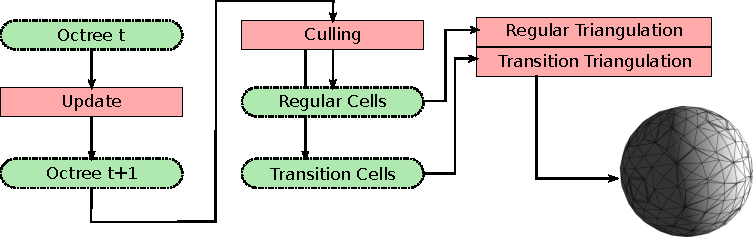
\includegraphics[width=0.9\textwidth]{pipeline}
  \caption{ This figure summarizes our GPU pipeline. Data buffers are represented in green and computations in red. Each computation retrieves data from a buffer and fills a new one. }
  \label{fig_pipeline} 
\end{figure*}

\paragraph{}
We present a new tool for isosurfaces visualisation that is adapted to rasterization issues and runs in real-time.
It is based on the adaptive triangulation of Lengyel \textit{et al}. \cite{lengyel2010voxel}, the linear quadtrees  of Gargantini \cite{gargantini1982effective}, and the LoD criterion of Dupuy \textit{et al.} \cite{dupuy2014quadtrees}.


\paragraph{}
Our pipeline is divided in 3 parts.
\begin{itemize}
\item The first step consists in updating a linear octree that maintains the active front of cells.
\item The second step performs both a culling on the octree cells, and creates the transition cells required for a crack-free MC triangulation.
\item The last step re-subdivides and triangulates the remaining cells.
\end{itemize}
This whole process is illustrated in Figure \ref{fig_pipeline}.
In the following sections, we present each step of our solution.

\subsection{Maintaining the linear octree}

Our method triangulates a set of cells.
Therefore, the first step of our pipeline evaluates a LoD criterion on each cell to determine if it is kept, split or merged.
In this section, we present the GPU representation for those trees, as well as the criterion we use to evaluate the new partition.

\subsubsection*{Linear octree on the GPU}

\begin{figure}
\centering
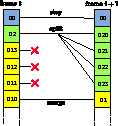
\includegraphics[height=0.2\textheight]{subdivision}
\caption{The octree at frame $t$ is stored as a list of Morton codes in a buffer. 
To update the tree, we fill a new buffer representing its state at frame $t+1$. 
On the GPU, each code of the first buffer is processed in parallel. 
If the cell is to be subdivided, it writes the codes of its children in the new buffer. 
If it merges, it writes either nothing, or the code of its parent (if it is the first child).
If it is kept, it just re-writes its own code. }
\label{subdivision}
\end{figure}

\paragraph{}
Dupuy \textit{et al}. \cite{dupuy2014quadtrees} proposed an implementation to handle efficiently quadtrees on the GPU.
Here, we want to manipulate an octree, hence, we generalize their solution to the third dimension.

\paragraph{}
To represent the cells, we use Morton codes.
Those codes are a succession of locations relatively to the root node.
In three dimensions, there are $2^3 = 8$ possible locations for a node so 3 bits are required to encode one subdivision.
Thus, if we keep the codes on 32 bits as in \cite{dupuy2014quadtrees}, we will be limited to a maximal subdivision depth of 9.
This is too coarse to do a correct triangulation of the surface.
Therefore, we used 64 bits for the encoding. 
This doubles the memory size of the front but, by using 5 bits for the depth of the cell and the other 59 bits for the code, we can subdivide 19 times.

\paragraph{}
At each frame we have the active front of the previous frame, $t$, and we want to update it to get the front at frame $t+1$.
To do so, we evaluate the LoD criterion given in equation (\ref{lod_criterion}) on every cell at frame $t$.
We then test the equations (\ref{split_test}) and (\ref{merge_test}) to determine if the cell should split or merge.
If a cell splits, it emits the codes of its children.
If a cell is kept it re-emits its own code.
If a cell merges, there are two possibilities.
If it is the first child (with the lowest Morton code), it emits the code of its parent.
Otherwise, it does nothing. 
This ensures that the merging operation produce only one cell.
The new cells are written into a new buffer that represents the active front at frame $t+1$.
This is illustrated Figure \ref{subdivision}.

\subsubsection*{Improved LoD criterion}

\paragraph{}
Dupuy \textit{et al.} manipulated quadtrees, a two dimensional structure, which contained a reasonable amount of cells in their active front.
This amount is greater when using an octree as those structures are in three dimensions.
We thus extended the LoD criterion determining the partition to minimize the size of the front.
Note that our extended criterion could still be used in two dimensions.

\paragraph{}
Here, we use the criterion given equation (\ref{lod_criterion}).
Its evaluation is data parallel and controls the projected size of the cells.
However, it is based on the Euclidean distance between a cell and the camera. 
Since this distance is absolute, cells behind the camera are highly subdivided even though they do not contribute to the final image.
Therefore, we combine this Euclidean distance with a radial angle to the camera's forward direction.
Cells behind the camera are then less subdivided, which reduces the number of cells in the octree.
The new criterion is given equation \ref{improved_lod_criterion} and illustrated Figure \ref{fig_lod_octree}.
\\
\begin{equation}
z'= z +
\begin{cases}
    w \cdot z \cdot (\theta - \alpha) 	& \text{if } \theta \geq \alpha\\
    0	              		    			& \text{else.}
\end{cases}
\label{improved_lod_criterion}
\end{equation}

\begin{figure}
  	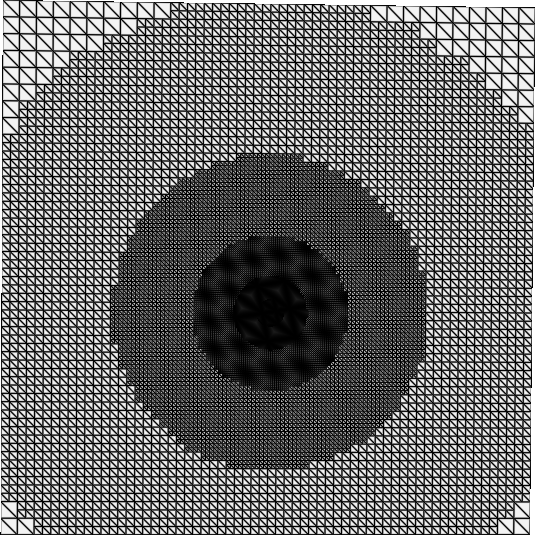
\includegraphics[width=0.4\linewidth]{viewlod1_small}
  	\hfill
  	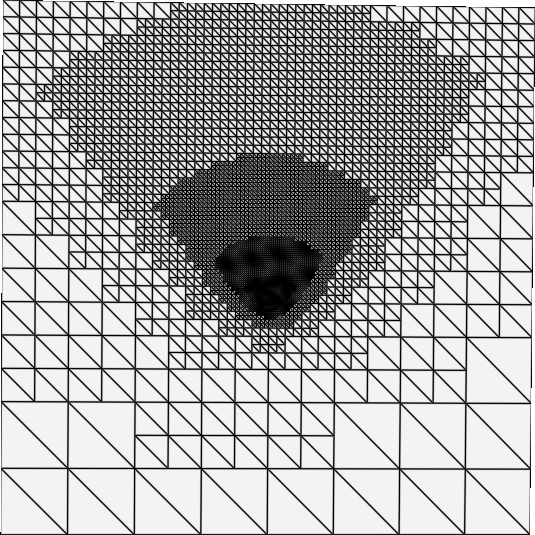
\includegraphics[width=0.4\linewidth]{viewlod2_small}
  \caption{ Adaptive triangulation of a plane. The camera is located in the center and looks up. (Left) uses the criterion in \cite{dupuy2014quadtrees} and (Right) uses our criterion.
  The total number of cells is (Left) 1037114 and (Right) 210323.}
  \label{fig_lod_octree} 
\end{figure}

\paragraph{}
In this equation, $z$ is the Euclidean distance between the center of the cell and the camera, $\theta$ is the angle and $\alpha$ is the fovy, both expressed in radians.
The parameter $w$ controls the importance of the radial distance over the Euclidean distance.
Its value has to be chosen carefully.
If it is too high, the difference of levels between the cells on both side of the frustum becomes very important, which might break the octree consistency. 
Empirically, we found that using $w \leq 6 $ prevents artefacts.

\paragraph{}
With this new $z'$, the criterion evaluated is now $s(z')$ instead of $s(z)$.
Note that we may lose the guarantee of maintaining a restricted octree outside the frustum.
However, as those cells are not triangulated, the visualisation is not impacted.

\subsection{Culling and transitions determination}

\paragraph{}
Once the active front has been updated, it contains the list of the cells to triangulate.
We then apply frustum culling to remove the nodes that are outside the view frustum.
We also remove empty cells; a cell that is fully inside or outside the object will not generate triangles and therefore should not be triangulated.
The remaining cells are stored in a new buffer that is used as input for triangulation.

\paragraph{}
If those cells are directly triangulated, cracks will appear at resolution changes.
As, Lengyel \textit{et al.} \cite{lengyel2010voxel}, we solve this issue by inserting and triangulating transition cells.
At each frame, we identify the level changes in the octree to create the corresponding transitions.
We do so by checking if a cell has a neighbour of higher resolution than itself.
%The difficulty is to do this with a data parallel method.
In our implementation, the chosen LoD criterion is fully data parallel and allows to determine if a cell has been split or merged.
Therefore, we can determine the transitions by evaluating this criterion on the neighbours of a cell.

\paragraph{}
Our LoD criterion is based on the projected size of a cell.
We thus need the position of the neighbours of the current cell.
This is easy to compute as we know the position of the cell and its size.
We then test each of them to determine if it has been split, using equation (\ref{split_test}).
If this test is verified, we emit a transition cell.
Note that each cell can then emit a maximum of 3 transitions, one for each axis.
We finally have two buffers containing the octree and transition cells.

\subsection{Triangulation and further subdivision}

\begin{figure}
  \centering
  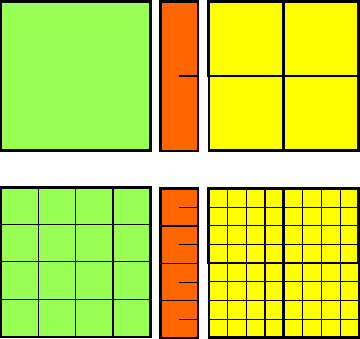
\includegraphics[width=0.6\linewidth]{tessellation}
  \caption{The upper configuration represents a cell with 4 more subdivided neighbours and a transition cell (red).
  This is what is returned by the update and culling steps.
  All those cells are subdivided, leading to the configuration presented on the bottom picture.
  Each cell has become a tile of $(2^N)$ cells on each dimension.
  Except for the transition cells, as their width do not change. }
  \label{tessellation} 
\end{figure}

\paragraph{}
We added a subdivision pass to increase the resolution of the extracted triangulation while staying real-time. 
When triangulating cells that are in the lowest levels of the octree, the resulting mesh is more precise. 
However, with a deeper octree, the update and culling steps are slowed down by the high number of cells to process.
We aim here at keeping the triangulation precise but with a coarser octree.

\paragraph{}
Therefore, a subdivision pass is added between the culling and the triangulation. 
It applies on every octree cell and on every transition cell.
Each octree cell is turned into a regular grid of smaller cells with a resolution of $(2^N)^3$, $N$ being a positive integer controlling the new level of subdivision.
The transition cells have a fixed width so they become a regular grid with a resolution of $(2^N)^2$ (Figure \ref{tessellation}).
This subdivision happens before the triangulation but after the LoD and culling.
This way, those first two steps run on a coarser octree, keeping their efficiency, while the triangulation is done on smaller cells, leading to a more precise mesh.

\paragraph{}
However, no culling is done on the new smaller cells.
Therefore, they will all be triangulated even if they are empty or outside the frustum. 
There is then a $N$ for which it is more interesting to cull a deeper tree than to subdivide the cells. 
Our experiments showed that the best $N$ is 2.

\paragraph{}
The last step is then to apply MC with the modified tables given by Lengyel \textit{et al.} to triangulate the cells and render our surface.
 %how/why it works
\section{Results}

We tested our method with an Intel Pentium 3550M processor and a NVIDIA GeForce GTX 850M GPU. 
We implemented it with C++ and GLSL. 
The pipeline runs with geometry shaders, combined with transform feedbacks. 

\paragraph{}
We ran our method on different volumetric datasets.
The first one is a stack-based representation of a terrain, called Moria, created with the ARCHES framework \cite{peytavie2009arches}.
It contains $512^3$ voxels, which we uploaded on the GPU using a 3D texture.
We also used two other datasets to further illustrate the performances of our method.
We first visualised a set of metaballs.
Those implicit surfaces are defined analytically to be evaluated on the GPU and are updated at every frame.
This scene creates objects that goes through high geometrical changes and thus cannot be precomputed.
We also visualised an animated ocean.
This object is again defined analytically and evaluated on the GPU. 
All those scenes are illustrated in Figure \ref{final_outputs} and in the accompanying video.

\paragraph{}
In all our experiments, we used the LoD criterion given in equation (\ref{improved_lod_criterion}).
This criterion is data parallel and is based on the projected size of the cells.
It thus prevents rasterization under-sampling and can be efficiently used on the GPU (Figure \ref{lod})

\begin{figure}
\centering
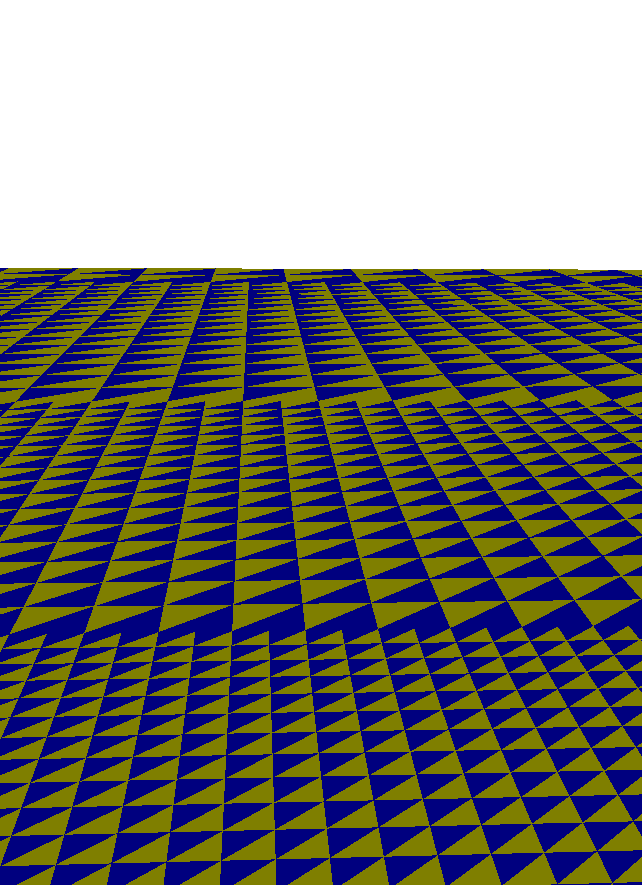
\includegraphics[height=0.2\textheight]{alias}
\hfill
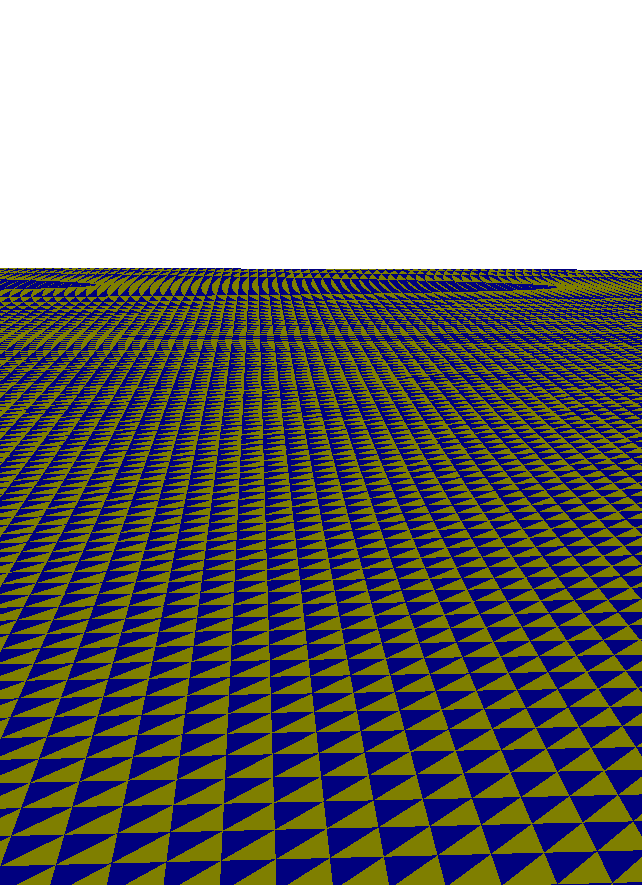
\includegraphics[height=0.2\textheight]{filtered}
\caption{Each extracted triangle has a different color. (Right) presents the result of rasterizing an object visualised with a regular grid. (Left) presents the result of rasterizing an object visualised with our LoD criterion. It can be seen that the aliasing artefacts present on (Right) disappeared on (Left).}
\label{lod}
\end{figure}

\subsection{Stack-based terrain}

\paragraph{}
We ran our method on the Moria scene \cite{peytavie2009arches}, enhanced with a noise function to add high resolution geometric details.
We present the average execution times for each step of the pipeline, as well as the number of cells in input (Table \ref{table_step}).

\begin{table}[tb]
\centering
\begin{tabular}{|l|c|c|c|}
\hline
Step           & Time (ms) & \#Cells & Memory (MB) \\ \hline
Update         & 1.13      & 219295  & 1.67        \\
Culling        & 3.3       & 219295  & 1.67        \\
Triangulation  & 0.94      & 5570    & 0.04        \\ \hline
Total GPU time & \multicolumn{3}{c|}{5.4}           \\ 
Total CPU Time & \multicolumn{3}{c|}{2.3}          \\ \hline
\end{tabular}
\caption{Average execution time for each step of the pipeline during a flythrough of the Moria scene.
The first column gives the average execution time, 
the second contains the number of cells in input, and
the last gives the memory size of the buffer used.
Since each cell is coded on 64 bits, the memory footprint of a buffer is $\mathrm{buffer\_size} * 64$ bits.}
\label{table_step}
\end{table}

\paragraph{}
We can note that updating the octree is very fast (less than 2 ms) whereas the culling step is slower (by roughly 300\%).
This is due to the fact that this pass runs tests on the whole partition, which can be computationally expensive.
Nonetheless, this efficient culling allows the triangulation to run on a very small amount of cells, thus reaching very good performances.
Finally, the total GPU time needed to update and triangulate the new frame is under 6 ms (180 FPS), for a memory consumption of only 4 MB.
Furthermore, as every computation is done on the GPU, the CPU is only active for 2 ms to initiate the shaders.

\subsection{Animated metaballs}

\paragraph{}
The cells inside the frustum are re-triangulated at each frame.
Therefore, it is possible to visualise fully dynamic data without any performance loss.
We tested this while visualising animated metaballs.
When running our experiments, the animation was stopped between the frames 5000 and 10000.
We can then show that our framerate is not affected by the changes in the scene.
The camera was static during the whole experiment to remove all variability that would have been induced if the number of cells to evaluate was changing.
The resulting graph is shown in Figure \ref{metaballs_graph}.

\begin{figure}
\centering
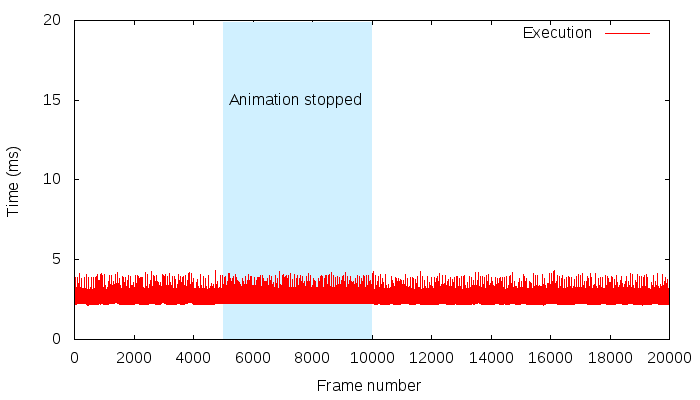
\includegraphics[width=\linewidth]{l_importance_d_etre_constant}
\caption{Rendering time for an animated scene. 
The average rendering time is about 3 ms even though the object is re-triangulated on each frame.
Those timings do not include the shading.
The blue box identifies the frames during which the object was static.
As can be seen, the fact that the object is or not animated has no impact whatsoever on the rendering time.}
\label{metaballs_graph}
\end{figure}

\paragraph{}
As can be seen on this graph, the triangulation timings are constant.
The only variability that can be measured is induced by the task scheduling on the GPU.


\subsection{Comparison}

%\paragraph{}
%Our goal in this work is to get a correct visualisation as fast as possible.
%The surface is triangulated for rasterization purposes and is not kept in memory.
%This differs from other methods that focuses on the topology of the mesh and return a full mesh.
%Furthermore, we gave ourselves the constraint that this method should be completely data parallel.
%This condition allows us to present a full GPU implementation with very high framerates.
%From those, we can afford to re-triangulate the whole object on the fly and still do a real-time visualisation.
%This differentiate our solution from most methods that achieve real-time through pre-process and data caching.

\paragraph{}
As developed during the introduction, there are several kind of methods on the state of the art.
The first category focuses on extracting a complete mesh from the data and are thus slower than methods that aim only at visualisation.
Amongst the visualisation solutions, the real-time is mostly achieved with data caching and pre-processing.
Here, we constrained ourselves to run in real-time without this data-caching and pre-processing, by taking full advantage of the GPU.
The solutions developed by other methods are thus quite different from ours.

\paragraph{}
We present a completely data parallel implementation based on the method of Lengyel \textit{et al}. \cite{lengyel2010voxel}.
Therefore, a pertinent comparison to prove our solution would be to compare both algorithms.
Since the method of Lengyel \textit{et al}. is part of a commercial game engine, it is not freely accessible.
We used instead a free implementation, independently developed by Lanner \cite{lanner}.
This implementation is based on data-caching.
The volumetric object is pre-triangulated at every level of detail during a preprocess.
Therefore during rendering, the only task left is to identify the cells of the octree's active front and to send their pre-computed triangulation to the GPU.
This increases the rendering speed but the preprocessing time can be prohibitive.
Furthermore, it is memory intensive.
Still, this implementation is very fast and allows localized modifications of the data.

\paragraph{}
We ran both methods on a static voxel based scene, adapting the LoD criteria to have a similar behaviour.
The dataset has a resolution of $256^3$.
The results are given in Figure \ref{cpu_gpu}.
It can be seen on this graph that even though we re-triangulate the cells at each frame, we are still running faster than a CPU implementation.
Furthermore, there is no transfer between the CPU and the GPU in our implementation.
This give us a speed up over CPU implementations that are constantly transferring data to the GPU.

\begin{figure}
\centering
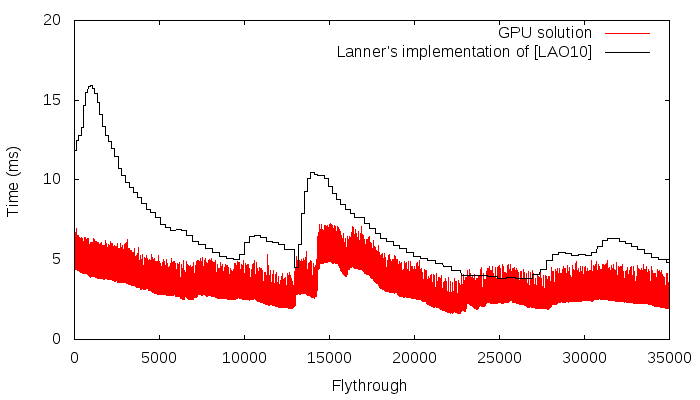
\includegraphics[width=\linewidth]{cpu_gpu}
\caption{Comparison between our GPU solution and Lanner's implementation \cite{lanner}.
This graph presents the execution time in ms for each frame.
}
\label{cpu_gpu}
\end{figure}


\begin{figure*}
\centering

\includegraphics[height=0.17\textheight]{metaballs}
\hfill

\includegraphics[height=0.17\textheight]{ocean}
\hfill
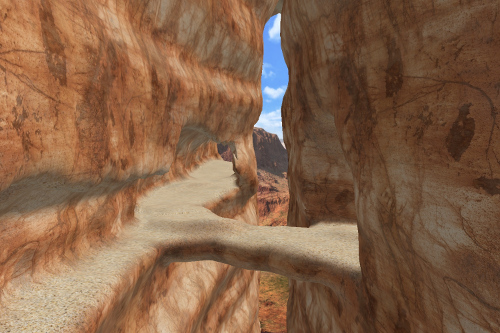
\includegraphics[height=0.17\textheight]{moria2}
\caption{This shows some outputs of our program. (Left) is an example of moving metaballs. (Middle) is an animated ocean. (Right) is a stack based terrain from the ARCHES plateform \cite{peytavie2009arches} }
\label{final_outputs}
\end{figure*}
 %how awesome it is
\section{Conclusion}

\paragraph{}
We presented a new tool for real-time visualisation of volumetric data.
Our method runs entirely and efficiently on the GPU.
We also triangulate the surface on the fly and therefore are able to visualize dynamic scenes such as moving metaballs.
Furthermore, with a LoD criterion that is based on the cells projected size, we prevent geometrical aliasing artefacts during rasterization.

\paragraph{}
One of the main characteristics of our solution is that it is based on MC.
Thus, it does a geometrical sampling of the object.
This implies that we can only render objects that can be sampled, \textit{i.e.} it prevents the rendering of frequencies that exceed by far the Nyquist limit.
To render such objects, ray casting based method are usually used.
Furthermore, the constant re-meshing of the object may also create popping artefacts, that could be fixed with vertex interpolation.

\paragraph{}
The choice of the LoD criterion could also improve this solution.
The actual one is based solely on the projected size of the cell. 
By combining it with the curvature of the object, we could limit the geometrical sampling issues.
However, this requires to be able to measure the curvature without pre process and with a data parallel algorithm.

 %how it could be more awesome

\bibliographystyle{alpha}
\bibliography{bibtex}

\appendix

\section{Ensuring a restricted octree}

\paragraph{}
To partition the space, Dupuy \textit{et al}. use the criterion given in equation (\ref{lod_criterion}).
They then test the size of the cell over this criterion.
If equation (\ref{ratio_division}) is verified, it means that the cell will be twice more subdivided than its neighbour.
To maintain a restricted tree, we need to ensure that it never happens.\\
\begin{equation}
\frac{\mathrm{cell\_size}}{2 \cdot s(z)} < 2k
\label{ratio_division}
\end{equation}

\paragraph{}
We illustrate this limit case Figure \ref{proof_constraint}.
Because the only variable is $\alpha$, we need to bound it.
From Thales, we can deduce:
$$
\frac{2k \cdot s(z)}{s(z)} = \frac{z + s(z)}{z}
$$
From this, we can express $z$ in terms of $s(z)$:
$$
z = \frac{s(z)}{2k - 1}
$$
Finally, trigonometry gives us:
$$
tan(\alpha) = 2k - 1
$$
As $\alpha$ is half the horizontal viewing angle, the octree is constraint as long as $\alpha < 2\arctan(2k - 1)$
For $k = 2$, this implies that the fovy must not exceed $142^o$.


\begin{figure} [h]
\centering
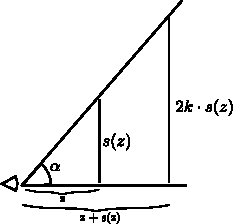
\includegraphics[height=0.2\textheight]{proof1}
\caption{If this situation happens, the LoD criterion no longer ensures to maintain a restricted tree.
The parameter $\alpha$ is thus bounded. Over a certain value, a cell can have two level of differences with its neighbours.
This figure is willingly wrongly scaled for readability purposes.}
\label{proof_constraint}
\end{figure}

\end{document}

